\documentclass{article}
\usepackage[margin=1.5in]{geometry}
\usepackage[T1]{fontenc}
\usepackage{graphicx}


\begin{document}
\ExplSyntaxOn
%% ==> cctab are global
% \cctab_new:N \g_my_cctab
% \cctab_gset:Nn \g_my_cctab {}  

%% ==> cctab scope
\section{cctab~ scope}
\cs_set_eq:NN \cctabend \cctab_end:
% 1. set to standard latex cctab
\cctab_begin:N \c_document_cctab  
hello world !
My hello 
\cctabend


% 2. restore to expl3 cctab
\section{cctab~ select}
\cctab_select:N \c_code_cctab
\par\prg_replicate:nn {2}{hello~ world\par}


% 3. char catcode set
\section{char~ catcode~ set~ and~ rescan}
% \char_value_catcode:n {65} = A
% see ASCII table: https://www.runoob.com/w3cnote/ascii.html
\cctab_const:Nn \g_my_cctab {
  \cctab_select:N \c_document_cctab
  \char_set_catcode_space:n {65}
}
% Rescan tokenlist VS normal Expl3
\tl_set:Nn \l_tmpa_tl {|A|B|A|C|$\alpha _1$|}
\tl_set_rescan:NnV \l_tmpb_tl { \cctab_select:N \g_my_cctab } \l_tmpa_tl
Under~ \LaTeX{}~ Catcode:\tl_use:N \l_tmpb_tl\par
Under~ Expl3~ Catcode:\tl_use:N \l_tmpa_tl\par
\ExplSyntaxOff

\section{ASCII~ Table}
\begin{center}
  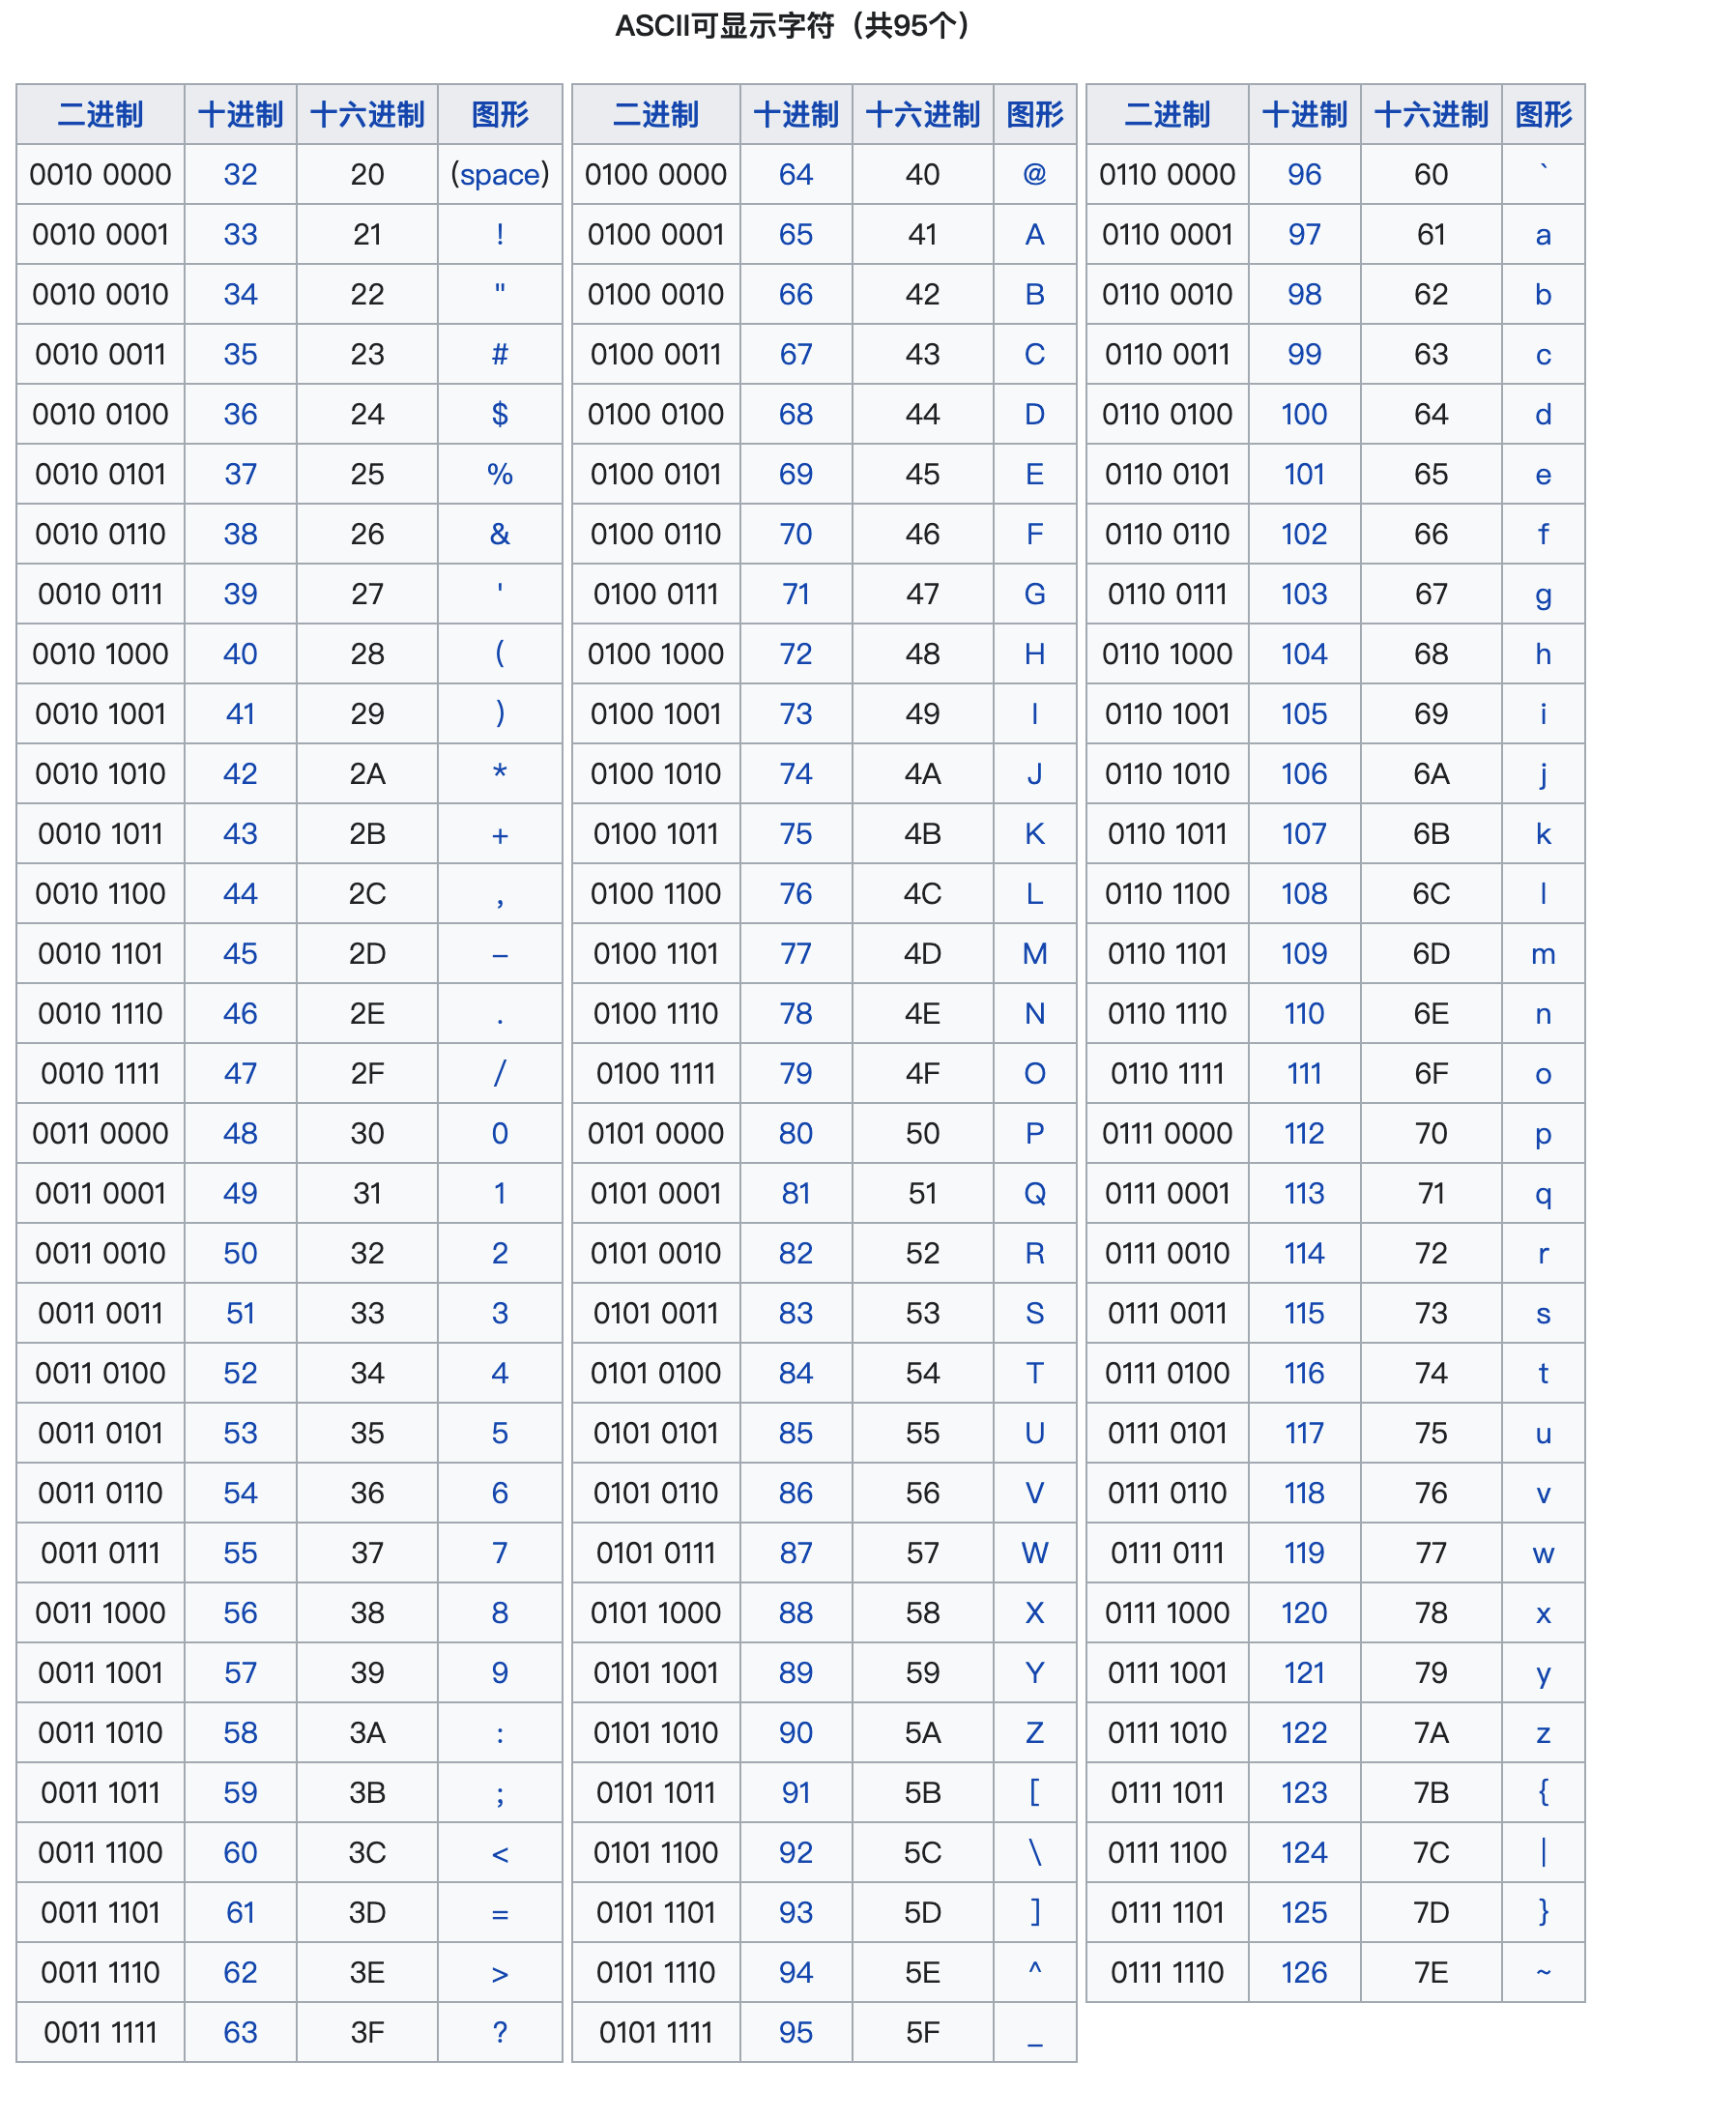
\includegraphics[height=.3\paperheight]{./ascii-1.png}
  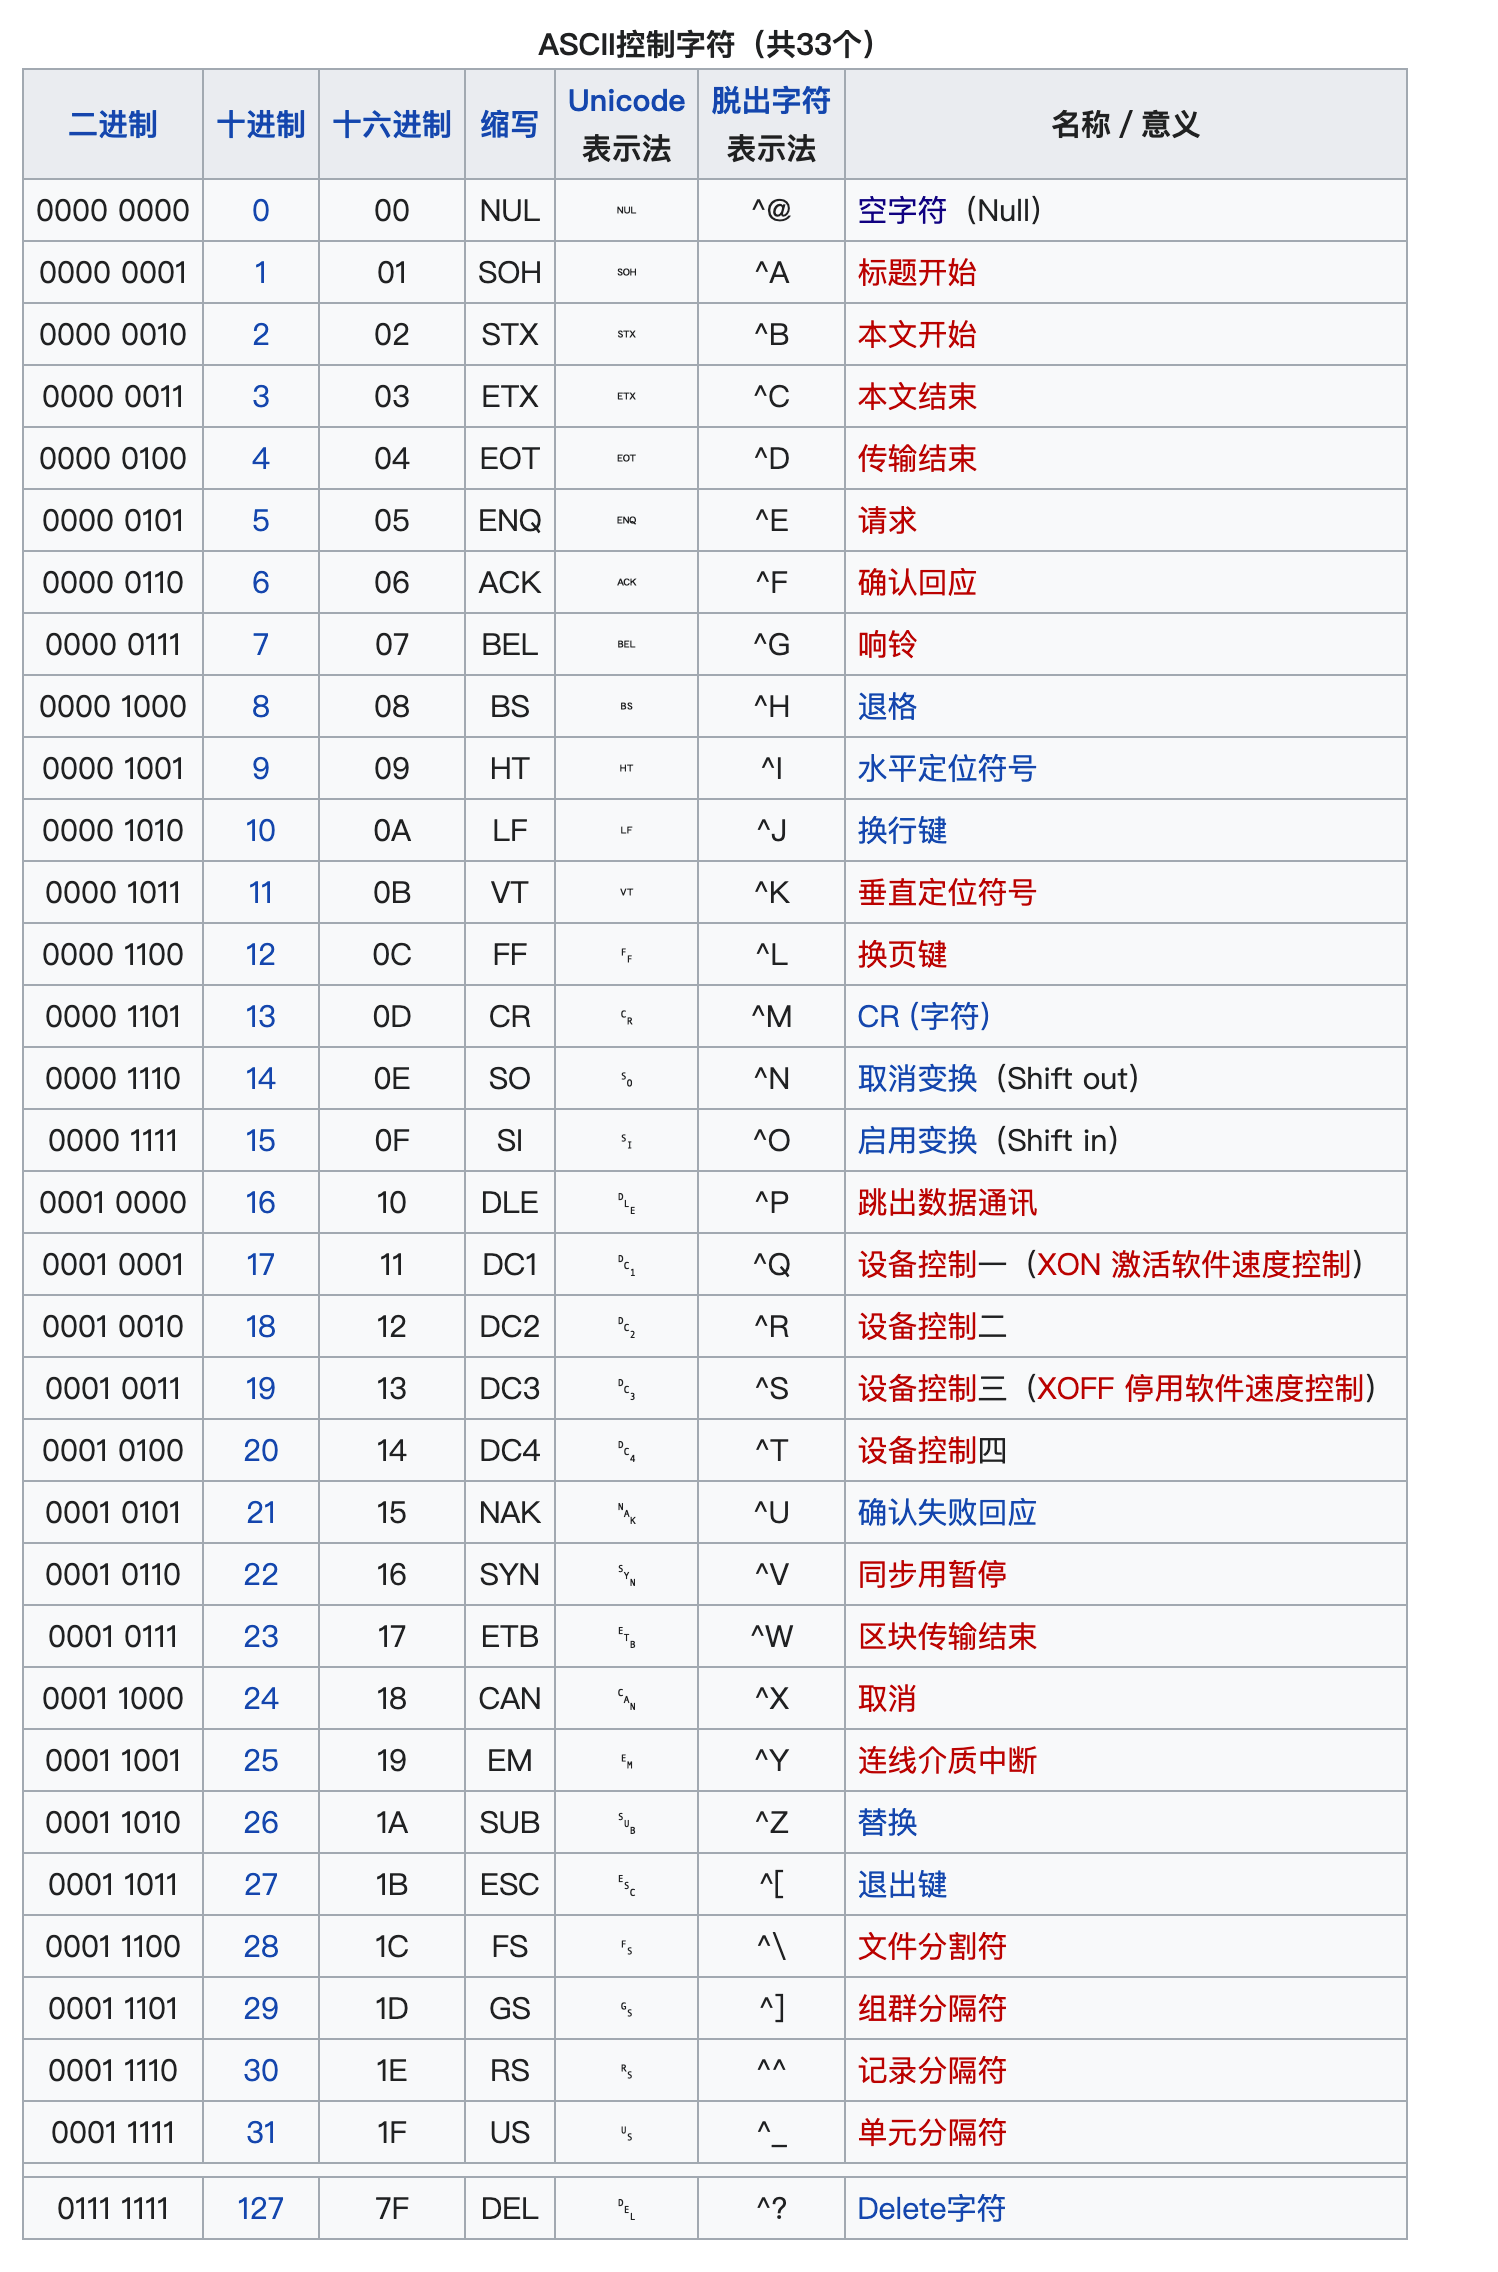
\includegraphics[height=.3\paperheight]{./ascii-2.png}
\end{center}

\section{App}
Appendix problem -- \verb|\endlinechar| and \verb|l3cctab|:\par 
\texttt{https://github.com/latex3/latex3/issues/611}
\end{document}


